\documentclass[runningheads]{comsis}

\def\journalissue{ComSIS Vol.~0, No.~0, December 2009}
\def\paperidnum{UDC, DOI: N/A}
\setcounter{page}{1}

\usepackage[dvipdfm]{hyperref}

\usepackage{amssymb}
\usepackage[fleqn]{amsmath}
\usepackage{hyperref}
\usepackage{graphicx}
\usepackage{semantic}
\usepackage{caption}
\usepackage{subcaption}

\title{Refactoring of Application Using Relational Database}
\author{Ondrej Macek\inst{1}}
\authorrunning{Ondrej Macek}
\institute{Czech Technical University in Prague\\
  Karlovo namesti 13 \\
121 35 Praha 2, Czech Republic\\
  \email{macekond@fel.cvut.cz}}

\begin{document}
\maketitle

\begin{abstract}
The change of application source code caused by refactoring affected not only the application, but it affect the stored data too if the persistent objects change. The change is usually processed in two steps: refactoring and data migration. We provide a solution capable to migrate database according to a refactoring in the application code. The feasibility of change and its data-secure processing is addressed too.

\vspace{6pt}\textbf{Keywords:} code refactoring, relational database, formal model
\end{abstract}


\section{Introduction}
\label{sec:intro}
The evolution (change) of a software is a common issue during software development. It occurs from many reasons in all phases of software lifecycle. The evolution severity usually depends on number of changes which has to be made and on the number of affected software components. Refactoring \cite{Fowler:Refactoring} is very popular practice in object-oriented environment for evolving the source code and software architecture. The evolution of database schema and stored data is implemented separately from  source code refactoring, although the change of application affects the database too. There exist object-relational mapping (ORM) frameworks, which can help with propagation of evolution from application to database. However these framework are usually not capable to solve complex refactoring cases nor migrate data properly as shown in Sect. \ref{sec:problem}.

%The focus of this paper is in data evolution context of software implemented in object oriented language using relational database. It means that the data evolution affect at least two software components: persistent objects (entities) and the database. The evolution is based on developer's point of view in this paper as it origins in the need to evolve code. This kind of evolution is straightforward in case there are no data stored in the database, because the database schema can be generated according to an evolved code, moreover some object-relational mapping (ORM) frameworks are able to process basic evolutionary transformation on database with stored data. The evolution of an software with ORM become more difficult when there are stored data and when the evolutionary scenario is more complex. The data migration to the new database schema is usually processed manually, which is expensive and error prone.

The problem of application and database evolution is discussed from developers point of view and the formal model of application refactoring and its impact is shown in Sect. \ref{sec:models}. There are introduced basic refactoring cases as well as the complex ones which are created as a sequences of the basic ones. The capabilities of proposed formal models are illustrated on the common refactoring issues in Sect. \ref{sec:case}.

%This paper shows how the application refactoring can be used as the source for database migration. The approach based on changes in code is useful in case when there is no model of database as it is derived directly from code. Next it can help developers to understand impact  of code changes on database. The formal description of code refactoring impact on database and stored data can help with construction of a standalone migration framework or evolutionary extension for existing ORM frameworks.

%The paper is organized as follows: first the evolution of software is described in detail in Sec. \ref{sec:problem}, then the related work in presented in Sec. \ref{sec:related-work}. In Sec. \ref{sec:models} the models of software and database is provided together with a set of basic evolutionary transformations. The impact of code refactoring on database is discussed in Sec. \ref{sec:evolution}. Finally the applicability and limitations of the proposed solution is discussed in Sec. \ref{sec:case}.

\section{Refactoring in Context of ORM} 
\label{sec:problem}
A software implemented using an object-oriented language, which uses relational database as a data storage consists of four main components. There is the application itself, the database schema, stored data and the object-relational mapping. The refactoring affects not only the application but the database too as the database has to be evolved when the persistent layer of the application changed to fit the object-relational mapping used in the software. The common current solution is based on capabilities of object-relational mapping frameworks which are capable to create a database schema according to the given source code or model. The process of evolution then proceed in following steps:
\begin{enumerate}
	\item The code is refactored (usually using the developers IDE).
	\item The ORM framework generates a new database schema.
	\item The data are migrated manually (if needed) from the old to the new database.
\end{enumerate}
The last step is error-prone as it is processed manually and the prone to error increases with complexity of refactoring. The evolution process require cooperation of a developer and a database administrator or it requires the developer has a knowledge of the database used by the software. The knowledge of the ORM is needed in both cases. Remarkable is the feasibility of data evolution has to be verified for each deployed software instance, because the data can differ. The data and information preservation is crucial issue of database evolution. Next observation is the evolution of the software is defined twice for one software - first for the application then for the database. 

\paragraph{Example 1} Let us have only two classes \emph{A} and \emph{B} in the application which are not connected by an association and there are corresponding tables \emph{tab\_a} and \emph{tab\_b} in the database, which contain data. We decide to inline \emph{B} into \emph{A}  during the development. The class \emph{A} contains all properties of \emph{B} and \emph{B} is removed from the application, the database schema is generated by the ORM framework and it contains only the table \emph{tab\_a}'. The data migration has to be created manually - the developer has to define the evolution twice. The mapping between data in \emph{tab\_a} and \emph{tab\_b} has to be provided to merge stored data correctly and impact of this mapping the database has to be verified: is there data which can be lost during inlining and is this lost intentional? 

\subsection{Solution Proposal}
We believe there exists better solution which automatize the process of database evolution according to the code refactoring. The solution is illustrated in the Fig. \ref{fig:evolution}. It is based on a change in the evolution process which assumes the ORM does not change during the evolution:
\begin{enumerate}
	\item The evolution of the whole software is defined independently on application or database.
	\item The evolution is interpreted for application and database.
	\item The evolution is executed.
\end{enumerate}
The process can decrease the human mistakes in the evolution process, because there is only one source for the evolution and the evolution is automatically interpreted for the application (as a refactoring) and database (as schema and data migration). The existence of the set of all possible software evolutions $E$ is based on a evolutionary transformations specific for application and database. Each transformation contains conditions of transformation feasibility, thus the feasibility of the evolution can be verified. 

% The evolution consists of change in application and in database as shown in the Figure \ref{fig:evolution}. 
\begin{figure}
\centering
	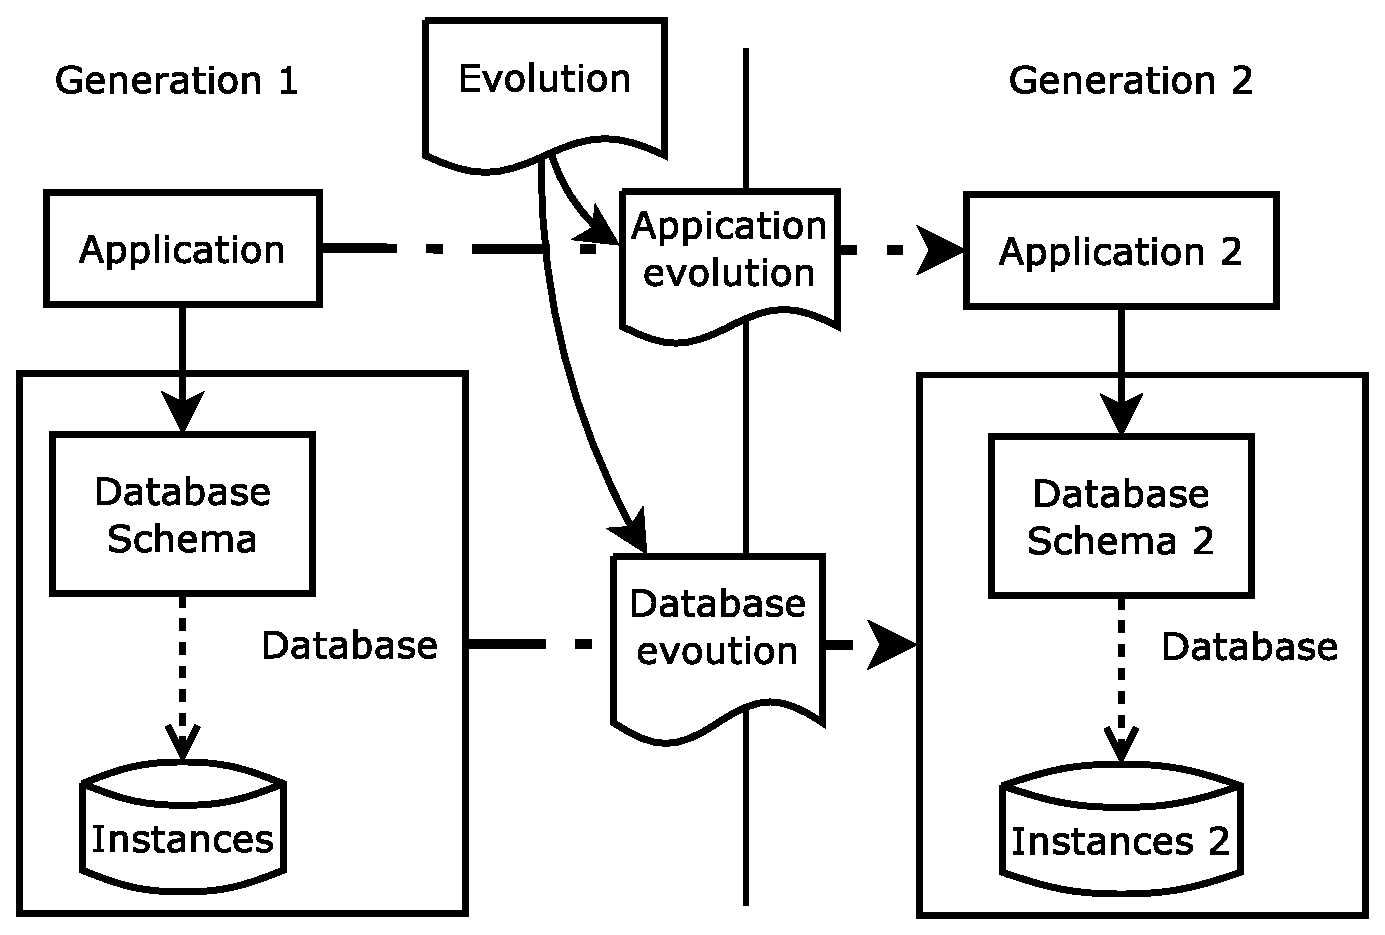
\includegraphics[width=.7\textwidth]{./images/evolution_simple}
	\caption{The evolution of data changes the system on all levels. The figure shows all the components of the evolution process.}
	\label{fig:evolution}
\end{figure}

The set $E$ is created with respect to the needs of a developer, therefore the evolutionary cases are similar to the refactoring cases. Nevertheless the refactoring itself does not provide enough information for the complex migration of database and data, therefore the inputs of transformation in $E$ are extended beyond normal refactoring inputs.

\paragraph{Example 2} The same situation from Example 1 can be solved more effectively if the \emph{inline} evolution is defined in $E$. All information needed for software evolution are provided as the input of the \emph{inline} transformation which is then automatically interpreted as inline of application classes and merge of tables on database level. The mapping is provided as the input of \emph{inline} too, thus the script for data migration can be generated. The structural feasibility is verified during the interpretation of the \emph{inline} and the migration script contains conditions which verifies the feasibility on level of data.

%The usual approach is to refactor code (which is quite fast due to help of IDE) and then re-generation or manual migration of the database. Another approach is to evolve a database (e.g. due to database optimizations) and then update the code. This approach is very common too, nevertheless this paper focus on evolution which origin from the application point of view. 

%The refactoring itself does not provide enough information for the complex migration of database and data, therefore a level defining the evolution is added - the set of all possible transformations $E$. The evolution definition from this level is propagated into both involved levels - application and database.



\section{Model of Software Evolution}
\label{sec:models}
The model-driven development (MDD) is a good approach to data evolution of various software components \cite{Moravec:PracticalApproach}. The software is represented by a set of models - application model and database model concretely. The evolution and ORM is represented by a set of model-to-model transformations and the interpretation of transformations from $E$ is a model-to-model transformation again. 


Three sets of transformations has to be defined to provide the capabilities described in Example 2: the set $E$ of all possible software transformations:
\begin{equation}
E = \{t | t: Software \rightarrow Software\}\:,
\end{equation}
the set of application refactorings:
\begin{equation}
A = \{t | t: Application \rightarrow Application\}
\end{equation}
and the set of database evolutionary transformations
\begin{equation}
 D = \{t | t: Database \rightarrow Database\}\:.
\end{equation}
The evolution of the software is defined as the interpretation of the transformation for each component of the software:
\begin{align}
& t(s) = \begin{cases}
software(\Psi(s, t), \Phi(s,t)) \; \mathbf{if} \; s \neq \perp \\\\
 	\perp
\end{cases}
s \in Software, t \in E \nonumber
\end{align}
Where $\Psi : E \rightarrow A $ interprets the software evolution cases to the code refactoring and $\Phi : E \rightarrow D $ interprets to the evolutionary transformation of database. The $\perp$ symbol denotes an inconsistent state of a software or its component. The definition of evolution allows to concatenate evolutionary transformations easily. 

\subsection{Software Model}
The software consists of three important components (as seen in Fig. \ref{fig:evolution}: application (its persistent layer concretely), database (consisting of database schema and stored data) and an ORM, therefore we define a software as a triple consisting of an application and a database which are connected together by an ORM.
The software has to be in consistent state so its users could have benefit from its usage. The software is in consistent state if application and database are consistent and the database structure corresponds to the application structure according to the ORM, therefore the the software is defined as:
\begin{align}
& software(a, d, \rho) = \begin{cases}
 software(a, d, \rho) \; \textbf{if} \; a \neq \perp \; \wedge \; b \neq \perp \\ \wedge \; \rho(a) = schema(d) 
 \\\\
 \perp
 \end{cases}\\
& a \in Application, d \in Database, \rho \in ORM \nonumber
\end{align}
The evolution of a software is a transformation from one consistent state to another one. These states are called generations of the software and the function which changed the state of a software are called transformations. 

%The main issue during the software evolution is the preservation of data and information consistency. The data lost is a situation when data are damaged or lost during the migration. The information consistency means the data was transformed according to the evolution of the application and they correspond with developer's intention. 

%The aim of this paper is to provide an definition of data evolution, which can be applied in case of various programming language, therefore the platform independent models of application and database are introduced. These models also provide simplification, which should increase the understanding of the proposed evolutions.

\subsection{Application Model}
Application is defined as a sequence of classes and it creates the context for all structures used in the software persistent layer:
\begin{align}
& \mathbf{Application} = (Class*) \\
& 	\mathbf{Class} = (label, Property*, Association*, Inheritance) \\
& \mathbf{Property} = (label, AppType, DefaultValue, \nonumber \\ & \;\;\;\;  Cardinality, Mandatory) \\
&	\mathbf{Association} = (label, classRef, startCardinality, endCardinality)  \\
& \mathbf{Inheritance} = (class, InheritanceType) \\¨
& \mathbf{InheritanceType} = SINGLETABLE \; | \; TABLE-PER-CLASS \\
& \mathbf{AppType} = APPSTRING
\end{align}

\paragraph{Class} Class represents a basic structural unit in the application model. It has a unique name, one or more properties and it can be associated to other classes in the application. The properties of a class can be of two kinds - values or collections - according of theirs cardinality.
	 
\paragraph{Property} Property represents a feature of a class which is represented as a primitive type. The property can be mandatory, can have a default value and according to its cardinality it can represent a single value or a collection of values. 

\paragraph {Association} Association represents a connection between two classes. It has a unique name and the reference is represented by the label of referenced class. The class which owns the association is consider to be the starting class of an association, referenced class is consider to be the ending class of an association. The cardinalities defines the multiplicity of both association ends.


\paragraph{Application type} Application type ($AppType$) represents primitive type in the application. There are usually defined types such as String, Integer, Boolean etc. in contrast there is only one type in our model, because we focus on structural and data changes and type casting operations are not important for us. The only $AppType$ type is called $APPSTRING$.

 There is not allowed multiple ancestors and of course a class can not be its own ancestor cyclically. We also assume there is only one type of inheritance type in the class hierarchy.



\subsection{Application Manipulation}
\label{sec:app-evolution}
The application model defines only the structure of an application thus there are defined transformation for its creating, altering and removing parts of the model (the set $A$). The conditions for successful transformations are simple in case of creating or altering:
\begin{enumerate}
	\item The name collisions has to be prevent when creating an class in the model or altering its name.
	\item All references have to be updated when renaming a class.
	\item The existence of referenced class has to be verified when creating or altering an association.  
\end{enumerate}
The only issue during deleting classes etc. from an application is the class can be removed only in case it is not associated by other classes. The transformations from $A$ are in table \ref{tab:app-evolution}. The list of altering operations is not complete as there are missing transformation for changing the obligation or cardinality of properties and associations. It is because these transformations are not so important for complex refactorings. 
\begin{table}
\caption{The transformations for application evolution.}
	\label{tab:app-evolution}
\centering
	\begin{tabular}{ll}
	\hline
	Type of transformation & Defined transformations \\
	\hline
	\\[-2ex] 
	Application Creation
	& newProperty(className, property, application) \\
	& newAssociation(className, association, mapping, \\ &  \hspace{0.5in}application) \\
	&  newClass(class, application) \\
	Application Alternation
		& renameProperty(className, oldName, newName, \\ &  \hspace{0.5in} application) \\
		& renameAssociation(className, oldName, newName, \\ &  \hspace{0.5in}application) \\
		& renameClass(oldName, newName, application)\\
		& changeReference(referncedClass, newReferencedClass) \\
		Application Disassembly 
		& removeProperty(className, propertyName,\\ &  \hspace{0.5in} application) \\
		& removeAssociation(className, associationName, \\ &  \hspace{0.5in}application) \\
		& removeClass(className, application)\\
%	Copy Structure
%		& copyProperty(sourceClass, property, targetClass,\\ &  \hspace{0.5in} newName, application)  \\
%		& copyClass(class, newName, application) \\
	Inheritance manipulation   & setParent(class, parentClass) \\
		& removeParent(childClass) \\
		& pushDown(class, property)\\
		& pullUp(class, property)\\
	\hline
	\end{tabular}
\end{table}

\subsection{Database Model}
The relational database consists of database schema which defines the structure of the database and data, which in the software represents stored instances. The database is defined as:
\begin{align}
&	\mathbf{Database} = ( Table*, Row* )\\
&	\mathbf{Table} = (label, primaryKey, Column*, ForeignKey*)\\
&	\mathbf{Column} = (label, DbType, DefaultValue, Constraint*) \\
&	\mathbf{ForeignKey} = (Label, Label, Constraint*) \\
&	\mathbf{PrimaryKey} =  ( Label, Sequence ) \\
&	\mathbf{DbType} = DBSTRING \; | \; DBINT\\
&	\mathbf{Constraint} = NOTNULL \; | \; UNIQUE 
\end{align}

\paragraph{Table} Table represents a basic concept of database schema. It has a unique name, one or more columns and it can be related to other tables in the schema by foreign keys. Rows in the table represents stored data.

\paragraph{Column} Column defines data values and types which can be part of a table record.

\paragraph{Foreign key} Foreign key is a reference to another table's primary key, it has an unique name and it can be constrained. The value of a foreign key is $\varnothing$ or a non-zero natural number.

\paragraph{Primary key} Primary key is unambiguous identifier of a record in a table. The primary key is always provided (automatically generated) by the database as a non-zero natural number. Primary key is always defined with constraints\\ $NOTNULL$ and $UNIQUE$. The sequence generates values of primary key. The new value of a key is obtained by calling the function $next(s)$. The sequence which provides numbers incremented by one is called $s_1$ if the increment is 1, $s_{10}$ if the increment is 10 etc.

\paragraph{Data Types} Database data types $DbType$ represents primitive types in the database. There are usually defined types such as Varchar, Integer, Boolean etc. There is only one type of column values defined in the model called \\ $DBSTRING$. Next the $DBINT$ type is defined for the values of keys.

\paragraph{Constraints} There are two types of constraints defined in the model. Both constraints are column constraints - first constraint defines non-empty columns, second constraint defines there has to be unique records in a column or foreign key.

\paragraph{Data} A database consists not only from schema but also from data which are represented as rows in a table. A table row in our model is a tuple consisting of value pairs, which represents concrete value of concrete column or key. Each row contains a name of a table it belongs to.
\begin{align}
&	\mathbf{Row} = (Label, Pair*) \\
&	\mathbf{Pair} = (Label, Value) 
\end{align}


\subsection{Database Manipulation}
\label{sec:db-evolution}
The database consists of two parts - from database schema which defines the structure and from stored data - hence the transformations from set $D$ have to consider both parts. The transformation for manipulation of structure has similar conditions to the evolution of application application. The transformations for data manipulation are inspired by the SQL language. The basic transformations are in Table \ref{tab:db-basic-evolution}. The set of transformations for database manipulation is limited in contrast with the SQL language as we mentioned only transformation necessary for data evolution on database level. 

\begin{table}
\caption{The transformations for database evolution. The transformations can be mapped to SQL intuitevly.}
	\label{tab:db-basic-evolution}
\centering
\setlength\tabcolsep{0.5em}
	\begin{tabular}{ll}
	\hline
	Type of transformation & Defined transformations \\
	\hline
	\\[-2ex] Database Creation
	& addColumn(tableName, column, database) \\
	& addForeignKey(tableName, key, database) \\
	& addTable(table, database)\\
	Database Alternation
	& alterColumnName(tableName, oldName, \\ & \hspace{0.5in}newName, dataabse) \\
	& alterForeignKeyName(tableName, oldName, \\ & \hspace{0.5in}newName, dataabse) \\
	& alterTableName(oldName, newName, dataabse) \\
	Database Disasembling
	& dropColumn(tableName, columnName, database) \\
	& dropForeignKey(tableName, keyName, database) \\
	& dropTable(tableName, database) \\
	Data Manipulation
	& select(tableName, rowId, database) \\
	& select(tableName, database) \\
	& insert(row, database) \\
	& insert(rowId, value, database) \\
	& delete(tableName, rowId, database) \\
	& delete(tableName, rowId, columnName, database) \\
	Copy Structure
	& copyColumnStructure(sourceTableName,\\ &  \hspace{0.5in} targetTableName,  sourceColumnName, \\ &  \hspace{0.5in} newName, database) \\
	& copyTableStructure(sourceTable, newTableName, \\ &  \hspace{0.5in} database) \\
	Copy Structure and Values
	& copyColumn(sourceTable, targetTable, \\
	& \hspace{0.5in} sourceColumnName, targetColumnName, \\ 
	& \hspace{0.5in} mapping, database) \\
	& copyTable(sourceTable, newName, database) \\
	Data-secure Database Elements &
	dropEmptyColumn(tableName, columnName, \\
	Removal & \hspace{0.25in} database) \\
	& dropEmptyForeignKey(tableName, keyName, \\ & \hspace{0.25in} database) \\
	& dropEmptyTable(tableName, database) \\
	\hline
	\end{tabular}
\end{table}


\paragraph{Copying Database Elements}The transformations for copying the structure of a column or table serves more as helpers for advanced evolution cases. The \emph{copyColumn} transformation contains a mapping between instances (stored data). The mapping to provides information which value from the source table rows is copied to which row in target table. The mapping is usually defined as: 
\begin{align}\label{eq:mapping}
&	mapping : select(ORM(sourceName), database) \nonumber \\ 
& \;\;\;\;\; \rightarrow  (select(ORM(targetName), database) 
\end{align}
The result of the mapping has to respect the constraints on column (e.g. $NULL$ cannot be inserted into a column with $NOTNULL$ constraint defined) The character of transformation depend on the feature of provided mapping. There occurs no data lost if the mapping is surjective.

\paragraph{Data-secure Database Elements Removal} The transformation for remove elements from the database can have fatal impact on the data preservation, therefore the set of transformations is extended by a data secure transformations for removing database elements. These transformations are not part of the SQL standard, although they can be implemented as database functions. These transformations creates a secure way to remove elements from the database as they drops empty structural elements only. 

\subsection{Object Relational Mapping}
The ORM is the only fixed point in the software model we use. The mapping is similar to the Hibernate mapping \cite{Hibernate} , thus a lot of developers should be familiar with it. The main ideas are: 
\begin{itemize}
	\item classes are mapped to tables,
	\item single properties are mapped to column or if the property is collection then the property is mapped to a table,
	\item associations are mapped to foreign keys or to tables if the association represents many-to-many  relationship,
	\item the primary keys are created automatically for each table,
	\item names used on application are mapped into the database schema (e.g. because possible name collision of application classes and names of database schema elements) 
\end{itemize}
%The ORM mapping is a function $ORM : Application \rightarrow Database $.

\subsection{Software Evolution}
\label{sec:sw-evolution}
The evolution of the whole software is described from the developer point of view, therefore the transformations use the names and elements from application context. The names of application elements and elements themselves have to be transformed into a database context - this is assured by the ORM.

\subsection{Basic Evolutionary Transformations}
\label{sec:sw-basic-evolution}
The evolution of the whole software is based on the atomic transformations specific for each software part, which are defined in Sec. \ref{sec:app-evolution} and \ref{sec:db-evolution}. This section introduces how these primitives can be used to manipulate the software elements.

The basic evolutionary transformations of the software are based on basic evolution of an application. These transformations has to respect the ORM, because properties and associations can be mapped as a column (foreign key respectively) as shown on the example of creating a new property: 
\begin{align}
& \Phi(newProperty(className, property, application)) = \nonumber \\
& \;\;\; =  \begin{cases}
  addColumn(ORM(className), ORM(property), database) \\\mathbf{if} \; cardinality(property \leq 1)  \\\\
  addTable(ORM(property), database) \\
  \mathbf{if} \; cardinality(property > 1)  
   \end{cases}
\end{align}

Mapping between basic evolutionary transformations is provided in the shortened way in table \ref{tab:sw-basic-evolution}, there is the basic application transformation and possible mappings on database level according to to the cardinality.  
\begin{table}
	\caption{The mapping between evolution of the application and database transformations. The  transformation connected with inheritance are in Sect.\ref{sec:inheritance}. }
	\label{tab:sw-basic-evolution}
\centering
	\begin{tabular}{ll}
		\hline
	Application Transformation & Database Transformation \\
	\hline
	\\[-2ex] 
	newProperty & \textbf{if} $cardinality \leq 1$ \textbf{then} addColumn \textbf{else} addTable \\ 

	newAssociation & \textbf{if} $cardinality \leq 1$ \textbf{then} addColumn  \textbf{else} addTable \\

	newClass & addTable \\
	renameProperty & \textbf{if} $cardinality \leq 1$ \textbf{then}  renameColumn  \textbf{else} renameTable \\

	renameAssociation & \textbf{if} $cardinality \leq 1$ \textbf{then} renameForeignKey \\ & \hspace{1in} \textbf{else} renameTable \\
	
	renameClass & renameTable \\
	removeProperty & \textbf{if} $cardinality \leq 1$ \textbf{then} dropEmptyColumn  \\ & \hspace{1in}\textbf{else} dropEmptyTable \\
	
	removeAssociation & \textbf{if} $cardinality \leq 1$ \textbf{then}  dropEmptyForeignKey \\ & \hspace{1in} \textbf{else} dropEmptyTable \\
	removeClass & dropEmptyTable\\
	\hline
	\end{tabular}
\end{table}
The transformations for data-secure removal are used as default removing transformations, although the classic drop- transformations can be used. This should lead to the more careful usage of removing transformations.

\subsection{Advanced Evolutionary Transformations}
\label{sec:sw-adv-evolution}
Advanced evolutionary transformations are based on the basic ones, they can be obtained as a concatenation of transformations. This means the complex transformations are limited in the same way as their basic components. All transformations from the set $E$ presented so far has the same input information for both application and database, whereas the advanced transformations usually needs a mapping between stored data (instances) as theirs input. 


\paragraph{Copy Property}
The $copyProperty$ creates a duplicate of a property in a given class. It can rename the property so it can be used for creating duplicates of a property in the property owning class. If the mapping is not provided the transformation creates only a structural copy of the property otherwise it copies the values too. Therefore the  $copyProperty$ transformation is the simplest way to manipulate stored data.
\begin{align}
& copyProperty(sourceClass, propertyName, targetClass, \nonumber  \\
& \; \; \; mapping, software) 
\end{align}
The  $copyProperty$ is the first transformation when an additional information has to be added to the usual code refactoring. It is because the $copyColumn$ transformation needs one more information to succeed - there has to be provided mapping between the source and target table to assure the data information consistency. %Moreover the source and target should have the same structure, type and constraints.
The transformation is interpreted for both software components - in case of the application a new property is added:
\begin{align}
& \Psi(copyProperty(sourceClass, property, targetClass, mapping, \nonumber  \\ 
&  \; \; \; software)) = newProperty(targetClass, property, application) 
\end{align}
in case of database the copy of a column or table is created according to property's cardinality and then values are copied:
\begin{align}
& \Phi(copyProperty(sourceClass, property, targetClass, newName, \nonumber \\ 
&  \; \; \; mapping, software)) = \begin{cases}
 coypColumn(ORM(sourceClass),  \\ \;\;\; ORM(targetClass),  \\ \;\;\;alterColumnName(ORM(property), \\ \;\;\; ORM(newName)), mapping, database) \\ \; \mathbf{if} \; cardinality(property) \leq 1 \\\\
 copyTable(ORM(Property), \\ \;\;\; ORM(newName))
 \end{cases}
\end{align}

\paragraph{Move Property}
The $moveProperty$ transformation is based on the $copyProperty$ transformation followed by the $removeProperty$ so its construction is easy. On the other hand special attention has to be paid to the provided mapping of instances, because it can cause data loses. The ideal case is when the mapping is surjective, then the transformation can not cause the lost of data. %On the other hand the situation when the mapping does not provides pairs for all rows in a source table can lead to data loss. 
\begin{align}
& moveProperty(sourceClass, property, targetClass, newName,\nonumber  \\
& \;\;\; mapping, software) = removeProperty(sourceClass, property, \nonumber \\
& \;\;\; copyProperty(sourceClass, property, targetClass, \nonumber \\ 
& \;\;\;newName, mapping, software))
\end{align}

\paragraph{Extract and Inline Class}
Extract and inline class are two opposite transformations. First of them extract a new class from an existing class, second of them moves data from one class into another. Both transformations can be composed from already mentioned basic trasnformations:
\begin{align}
& extract(sourceClass, newClass, property*, software) = \nonumber  \\ 
& \; \; \; = moveProperty(sourceClass, newClass, property*, mapping \nonumber \\ 
& \; \; \; addClass(newClass, software))
\end{align}
The \emph{mapping} cannot be created according to the definition \ref{eq:mapping}, because there are no stored data in the table representing the \emph{newClass}, therefore the \emph{mapping} is defined as identity in case of \emph{extract}, therefore the rows in the new table has same primaryKey value as in their source class. The \emph{extract} transformations assumes the \emph{sourceClass} and \emph{newClass} has the same type of primary keys sequence. 
\begin{align}
& inline(targetClass, classToInline, mapping, software)) =  \nonumber \\
& \; \; \; = removeClass(classToInline, moveProperty(classToInline, \nonumber \\
& \; \; \; targetClass, properties(classToInline), mapping, software))
\end{align}


\paragraph{Merge Classes}
There occur situations when there is a need to merge two classes and the inlining transformation cannot be used because of name collisions among properties in such a case the $merge$ transformation can be used. \begin{align}
& \Psi(merge(firstClass, secondClass, newClassName, software)) = \nonumber \\
& \; \; \; = removeClass(secondClass, removeClass(firstClass,\nonumber  \\
& \; \; \; changeReference(secondClass, newClassName, \nonumber \\
& \; \; \; changeReference(firstClass, newClassName,\nonumber  \\
& \; \; \; addClass(class(newClassName, \nonumber  \\
& \; \; \; \; \;properties(firstClass) \cup properties(secondClass), \nonumber  \\
& \; \; \;\; \;associations(firstClass) \cup associations(secondClass), \nonumber  \\
& \; \; \;application)))))) 
\end{align}
The interpretation for the database level is more complicated as the transformation copies rows from different sources with different primary key sequences in the new (empty) table. Therefore the primary keys from origin instances has to be replaced by a new ones and all references (foreign keys) has to be updated accordingly. Next the \emph{merge} can be used only if the structure of classes and corresponding tables is the same or if the extra columns (foreign keys) are not constrained, because we are not able to automatically solve the  duplicity of values or missing values.

\subsection{Inheritance Manipulation}
\label{sec:inheritance}
The inheritance is important part of object-oriented world. The impact of change of this relationship to the database depends on the type of inheritance mapping similarly as in the case of \emph{moveProperty}. The \emph{setParent} transformation is described as example:
\begin{align}
&\Phi(setParent(childClass, parentClass)) = \nonumber \\
&= \begin{cases}
mergeTables(ORM(childClass), ORM(parentClass),\\
addColumn(column("inheritanceType", DBSTRING, "parentClass", \\ \; \; NOTNULL) ORM(parentClass), \\
     addColumn(column("inheritanceType", DBSTRING, "childClass", \\ NOTNULL) ORM(childClass), database))) \\
     \mathbf{if} \; inheritanceType = SINGLETABLE 
     \\\\
     addForeignKey(foreignKey("parent", ORM(parentClass), \\
     \; \; (NOTNULL, UNIQUE)), ORM(childClass), database) \\
     \mathbf{if} \; inheritanceType = TABLE-PER-CLASS \\ \wedge  
     isEmpty(ORM(childClass)) \wedge isEmpty(ORM(parentClass))
 \end{cases}
\end{align}
The inverse transformation \emph{removeParent} moves all columns from the parent table to the child table if there are data in the parent table, then the parent can be removed securely. This does not cover the case when the information from parent are not needed in its child, such as transformation has to be defined in several steps. 

Next transformations connected with inheritance are \emph{pushDown} and \emph{pullUp}. Pull up moves a property from child to parent so the \emph{moveProperty} can be used, the mapping of instances is based on the parent-child relationship. It means the column cannot be constrained with $NOTNULL$ constraint if there are more siblings in the hierarchy. The \emph{pushDown} transformation works in opposite direction. The easiest situation is where there no sibling in the hierarchy, then the \emph{moveProperty} can be used, otherwise we assume there are no stored data in the siblings. It is because the change of parent changes affects the instances of its children, when a property is moved only into one children the information consistency is violated, therefore we forbid such transformation, because we cannot anticipate developers intents.

The next two inheritance-related transformations are \emph{extractParent} and \emph{extractCommonParent} serves for extracting a parent class in based on given set of property from a class or from a couple of classes. The transformation is based on the \emph{extractClass} (and \emph{mergeClasses} in the second case). 




\section{Example of Usage}
The examples demonstrate how the transformations help with data evolution in real example of software evolution. There are two classes in our software $Person$ and $LegalParty$ both of them contains information about address (street, city and zip code) as shown in the Fig. \ref{fig:case1} where the database tables are shown. 

To improve the design of code the class Address has to be created which associated with both original classes and contains the data already stored in the software. 
\begin{figure}
\begin{subfigure}[b]{\textwidth}
	\centering
	\begin{tabular}{| c | l | l | l | l | }
	 	\hline
		Id &  Surname & Street & City & ZIP  \\ \hline  
		11 & Jackson & Central Park St & New York & 100 01  \\ \hline
		12 & Clooney & S Orange Ave & Orlando & 320 24  \\ \hline
	\end{tabular}
	\caption{Data stored in the table $Person$.}
\end{subfigure}
\begin{subfigure}[b]{\textwidth}
	\centering
	\begin{tabular}{| c | l | l | l | l | c |}
	 	\hline
		Id &  BusinessName & Street & City & ZIP \\ \hline  
		100 & Tools \& Machines & Olive ave. & New York & 100 01 \\ \hline
		200 & AI Robotics & Pine ave. & LA & 900 03  \\ \hline
	\end{tabular}
	\caption{Data stored in the table $LegalParty$.}
\end{subfigure}
	\caption{The initial state of the example used in the case study. There is a repetition of information structure in the $Person$ and $LegalParty$ class.}
	\label{fig:case1}
\end{figure}
The first  step of is to extract two temporary classes representing address of a $Person$ or of a $LegalParty$:
\begin{align}
s' &= extract("LegalParty",  "Address\_tmp2", "street", "city", "zip", \varnothing, \nonumber  \\ 
& \;\;\;\; extract("Person", "Address\_tmp1", "street", "city", "zip", \nonumber \\ & \;\;\;\;  \varnothing, software)))
\end{align}
Temporary classes has to be connected with the origin classes by an association. The associations are creates as optional because foreign key constrained with $NOTNULL$ can cause problems in the next phase of evolution.
\begin{align}
 s'' &= newAssociation("LegalParty", association("address", \nonumber \\
& \;\;\;\; "Address\_tmp2", 0, 1), mapping_2, \nonumber \\ & \;\;\;\; newAssociation("Person", association("address",\nonumber  \\
& \;\;\;\; "Address\_tmp1", 0, 1), mapping_1, s')))
\end{align}
The $mapping_1$ and $mapping_2$ can be defined using the equality of primary keys values, because the temporary classes were extracted from the $Person$ and $LegalParty$. Finally the temporary class are merged into one:
\begin{align}
 s''' &= merge("Address\_tmp1", "Address\_tmp2", "Address", s'')
\end{align}
The merge of classes is possible because the associations (and corresponding foreign keys) created in the previous step are not constrained. The result of the transformations is in the Fig. \ref{fig:case2}. 
\begin{figure}
\begin{subfigure}[b]{0.45\textwidth}
	\centering
	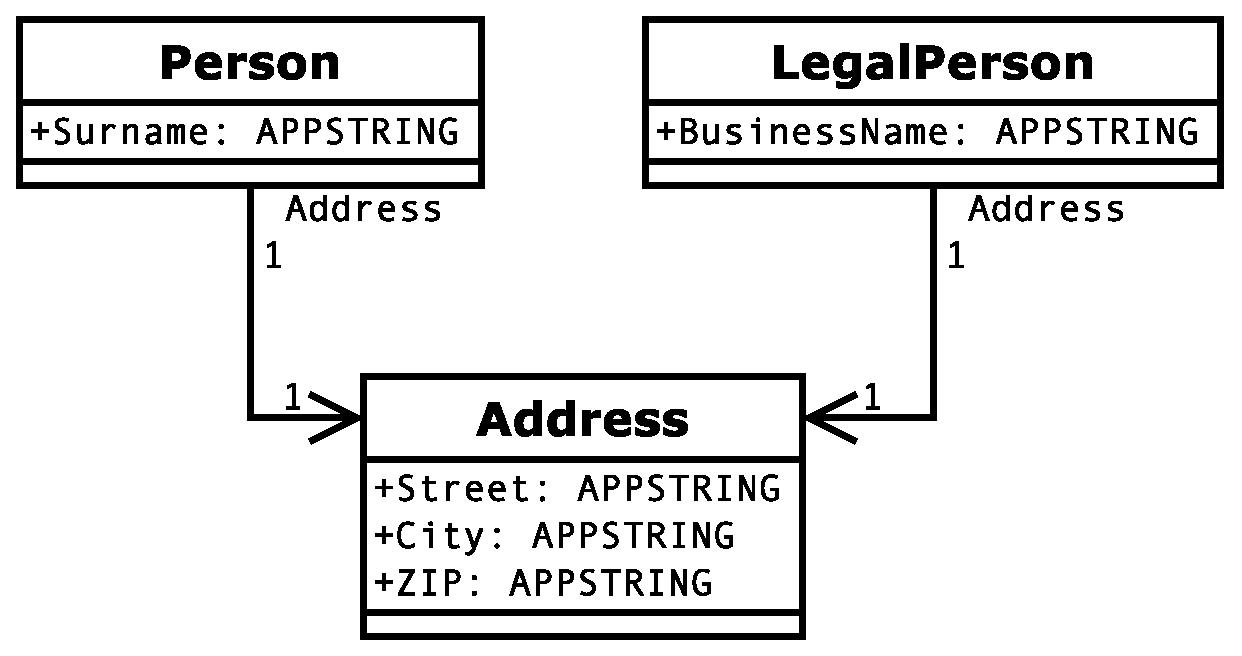
\includegraphics[width=\textwidth]{./images/case_app_9}
	\caption{The application model.}
\end{subfigure}
\quad
\begin{subfigure}[b]{0.45\textwidth}
	\centering
	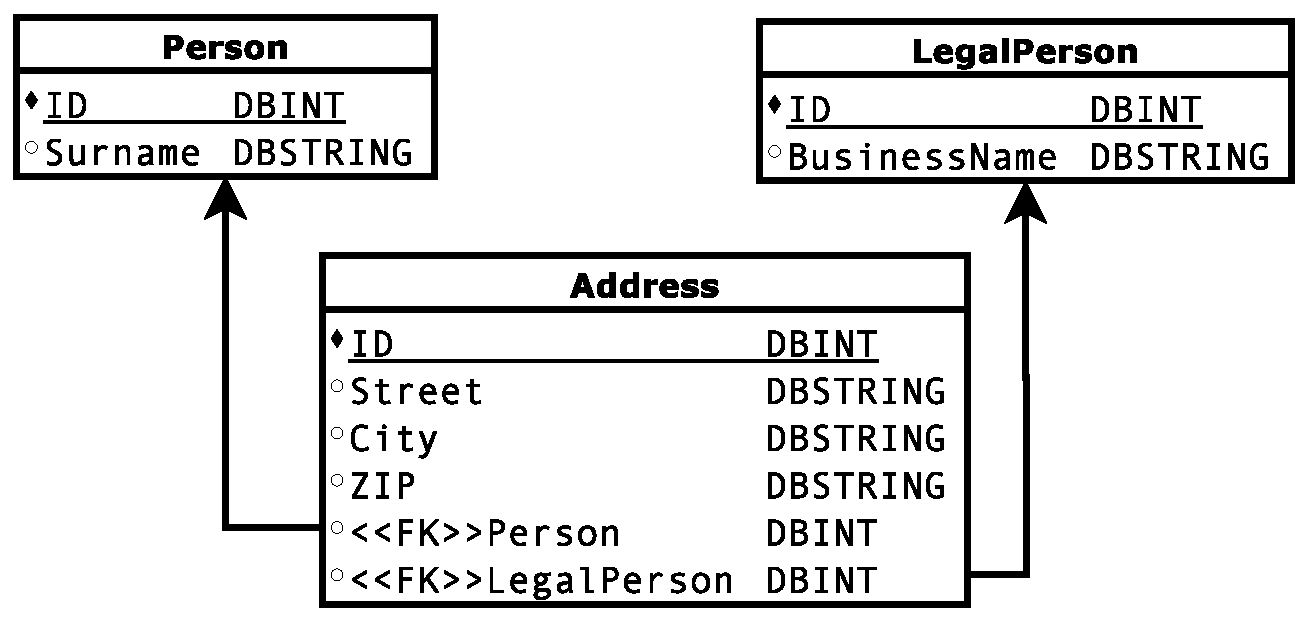
\includegraphics[width=\textwidth]{./images/case_db_8}
	\caption{The database model.}
\end{subfigure}
\begin{subfigure}[b]{\textwidth}
	\centering
	\begin{tabular}{| c | l | l | l | l | l |}
	 	\hline
		Id & Street & City & ZIP & Person\_Address & LegalParty\_Address\\ \hline  
		1 & Olive ave. & New York & 100 01 & & 100 \\ \hline
		2 & Pine ave. & LA & 900 03 & & 200  \\ \hline
		3 & Central Park St & New York & 100 01 & 11 &  \\ \hline
		4 & Orange Ave & Orlando & 320 24 & 12 &\\ \hline
	\end{tabular}
	\caption{Data stored in the table $Address$.}
\end{subfigure}
	\caption{The final state of the example used in the case study. There is only one table containing all addresses in the system, which reference the $Party$ and $LegalParty$.}
	\label{fig:case2}
\end{figure}
The change of the code can continue e.g. by adding more addresses to the $Person$ class, creating an enumeration for cities etc.

The example shows that defined transformations are able to perform regular data evolutions. It shows that usage of the transformations are sometimes not intuitive for user (e.g. creating temporary classes before merge), therefore next complex transformations has to be define based on user experience. The examples shows that the column constraint s often decide the feasibility of a transformation. 

\section{Capabilities of the Proposal}
\label{sec:case}
It is obvious that the set of defined transformation is limited because of focus on data preservation or transformation concatenation. On the other hand defined transformations are strong enough to handle a lot of refactoring cases. To verify this we use refactoring cases based on the Eclipse foundation refactoring statistics \cite{Eclipse:Refactoring} (the transformation influencing data chosen only) and on Fowler's book \cite{Fowler:Refactoring}. Selected refactorings are:
\begin{enumerate}
	\item \textbf{Rename} is the most used refactoring used according to Eclipse statistic and it is one of the basic refactoring cases introduced in the Sec. \ref{sec:sw-basic-evolution}.
	\item  \textbf{Move} refactoring is used in Eclipse to move properties from a class to another class within an inheritance hierarchy or to move classes between packages. In contrast our model does not consider packages, on the other hand it is able to move property from one class to another according given mapping, which contains not only move in hierarchy but a lot of other cases too.
	\item \textbf{Extract Class} is often used refactoring in Eclipse and it is mentioned in Fowler's book too. It is introduced as an example of advanced refactorings in Sec. \ref{sec:sw-adv-evolution} together with its opposite transformation $inline$.
	\item \textbf{Move field} from the Fowler's book is introduced as $moveProperty$ in Sec. \ref{sec:sw-basic-evolution}.
	\item \textbf{Replace Data Value with Object} is a refactoring case which is not mentioned among the evolutionary transformations, on the other hand it can be composed from already defined transformations:
	\begin{align}
& replaceDataWithObject(sourceClass, property, newObject, \nonumber \\
& \; \; \; software) = removeProperty(sourceClass, property, \nonumber \\
& \; \; \; newAssociation(sourceClass, newObject,  mapping,\nonumber  \\
& \; \; \; copyProperty(sourceClass, property, newObject, \nonumber \\ & \; \; \;  software)
	\end{align}
Where the mapping use the values copied in the first transformation as a matching point for creating connection between the old and the new class.
\end{enumerate}
The transformations proposed in this paper are able to implement all data refactorings used on Eclipse platform. There are some refactorings from Fowler which are not considered in the proposal: replace array with object, change unidirectional association to bidirectional (and reverse) and operations which replace types with polymorphism. However the proposal solves the most used refactorings.



\section{Related Work}
\label{sec:related-work}
Research of data and database evolution is not limited to relational ones only, there are also works in the areas of object databases and XML databases. These works provide solutions specific to concrete types of databases using various ranges of solutions - domain specific languages \cite{SERF}, extensions of existing standards or MDD \cite{Evolution_vs_Reorganization} or formal specification \cite{Tresch:1991vi}. These solutions are inspiring, however the domain of the ORM has its specific issues, so a solution from another domain has to be adapted carefully.

\paragraph{Informal definitions} The taxonomy of relational database evolution based on the entity-relationship model  is proposed in \cite{Roddick:TaxonomyOnERM}. The evolution is described as a change in entity-relationship model and change in relational database.  The semantics change patterns in context of conceptual schema is described in \cite{Wedemeijer:SemanticChangePatternsInConceptualSchema}, although its impact on database schema or data is not described. The main cases of data evolution are defined in both publications, however the description is informal. The extensive set of possible database refactorings is provided in \cite{Ambler:DbRefactoringBook}, where both schema and data evolution is discussed. The refactorings are intended to be used by database administrators, thus it assume database-first approach to evolution whereas this proposal is application-first.   

\paragraph{Formal frameworks} A general formal framework for database evolution is defined in \cite{McBrien:formal-framework-transformation}. The framework is based on a set of basic graph transformations which are then extended to transformations of the entity-relationship model. The framework and the defined transformations can be implemented in our proposal too. The contribution of the formal framework is definition of equivalent structures in relational database schemas. Our proposal is aimed to be used in domain of object-oriented languages where the class model is more common than entity-relationship model which is respected in our proposal. 

The formal definition of MDD approach to database schema evolution is proposed in \cite{Aboulsamh:FormalModelingEvolution}, where a changes of database conceptual schema is interpreted on both physical schema and data. In contrast our proposal is aimed to solve the problem of code refactoring and its impact on relational database, next we propose more complex transformations (such as \emph{copyProperty} or inheritance-related transformations) and examine the impact of platform specific constructs (such as foreign keys or constraints) on the evolution. 

A categorical framework for migration of object-oriented systems is proposed in \cite{Schulz:CategoricalModel}. This framework defines the refactoring of objects, data and methods, which are the main objectives of the framework. The impact of the object change on a relational database is not considered in the paper as it is aimed at object-oriented systems only.

\paragraph{Forward Round-Trip Engineering in Data Evolution} A round-trip approach for data evolution was described in \cite{VanPaesschen:2005to}, which was implemented in the SELF language. This approach proposed a forward-oriented evolution on all application levels in the software application. In contrast with our framework, the round-trip approach does not care about stored data because it is focused only on create, update and delete types of evolution.

A meta-model based approach to data evolution is proposed in \cite{Aboulsamh:MetaModelBasedApproachToIsDataEvolution} and very similar solution for data evolution is proposed, which is based on extended UML meta-model. The solution provides similar capabilities of change of application and database as does our proposal. In contrast our work is created with respect to ORM domain and therefore we extended the application meta-model with constructs typical for this domain.

\paragraph{ORM Frameworks} There are many object-relational mapping frameworks available for developers, and some of them provide tools for database migration. Hibernate \cite{Hibernate} is one of the most popular ORM frameworks in the Java community which is capable of creating a new table or adding a new column according to a change in the application. Active Record \cite{Active_Record} is an ORM framework in the Ruby on Rails environment. Since its first version it has contained support for database evolution according to the create-update-delete principle, in the form of so-called migrations \cite{Rails:Migrations} which can be extended by adding user SQL commands. Entity Framework \cite{Entity_Framework} is Microsoft's ORM solution for the .NET platform. Its capabilities of data evolution support are similar to those of Active Record. Neither of the frameworks is capable of automatization of complex refactoring cases.

\paragraph{Tools for Database Evolution} The MeDEA project \cite{Meda:Main} offers a tool for evolution of both database schema and stored data based on model-driven approach. The project DB-MAIN \cite{Hick:DBMAIN} provides a MDD approach to data evolution on all the levels of software we do. The project DB-MAIN is well documented formally. The PRISM is a research project for data management under schema evolution \cite{PRISM} in contrast with our proposal, and with MeDEA, it extends the SQL command set by so-called schema modification operators which implements the schema evolution.  Very promising solution is Liquibase \cite{Liquibase} a tool for database refactoring and evolution. It is capable to migrate both database schema and stored data. The evolution is described in a form of a XML document which can be interpreted on various databases. 

The difference between these frameworks and our proposal is that each has a different focus. All mentioned projects are aimed to  be used by database administrators; whereas our focus is on entities evolution, which is then propagated to a database with an emphasis on automatization. Our goal is to hide the entire database level from our users.

The project IMIS \cite{Bordbar:ModelBasedMigration} follows the same idea of applying MDD into evolution of a whole software, but does not provide a formal model or an overview of capabilities (defined transformations).

\section{Conclusion}
We discuss the impact of application refactoring on relational database schema and stored data. We introduce basic transformations of application and database, next show how the complex refactorings can be constructed based on basic refactorings. The transformations presented are capable to solve the main refactoring cases and provide both verification of transformations structural feasibility and data-secure migration for database schema and data. 

The proposal is based on the idea of MDD which is implemented by a set of models and transformations rules. This allows to simulate the behavior of an evolution in the platform independent environment.

The main contribution is the new point of view on the application refactoring. The application code and relational database co-evolution can improve the capabilities of IDEs and speed up the work of developers. Next contributions are definitions of impact of advanced refactoring cases on relational database and stored data.

\bibliographystyle{splncs03}     
\bibliography{references}   

\end{document}
